\section*{Supporting information}

\begin{figure}[h!]
\includegraphics[width=0.5\textwidth]{ncbi/out/ncbi.png}
\centering
\caption{\textbf{Cumulative number of different eukaryotic genomes annotated by NCBI.}}
\label{sfig:ncbi}
\end{figure}

\begin{figure}[h!]
\includegraphics[width=\textwidth]{clusters/out/clusters.png}
\centering
\caption{\textbf{Statistics of orthologous groups.}
\textbf{(A)} Each species is equally represented in orthologous groups (OGs). \textbf{(B)} A plurality of orthologous groups contain all species. \textbf{(C)} Nearly all proteins are associated with a single orthologous group. \textbf{(D)} The number of orthologous groups associated with a species is strongly correlated with the number of unique annotated proteins, which suggests the annotation pipeline generally identifies conserved genes.}
\label{sfig:clusters}
\end{figure}

\begin{figure}[h!]
\includegraphics[width=\textwidth]{paralogs/out/paralogs.png}
\centering
\caption{\textbf{Addition of paralogs to orthologous groups.}
\textbf{(A)} Most orthologous groups (OGs) have no in-paralogs. \textbf{(B, D)} Of the groups with paralogs, most have fewer than five. \textbf{(C)} The in-paralogs are generally only a small fraction of the sequences in an orthologous group.}
\label{sfig:paralogs}
\end{figure}

\begin{figure}[h!]
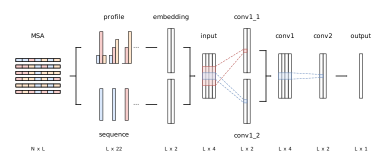
\includegraphics[width=\textwidth]{cnn_architecture.png}
\centering
\caption{\textbf{CNN architecture.}}
\label{sfig:cnn_architecture}
\end{figure}

\begin{figure}[h!]
\includegraphics[width=\textwidth]{cnn_training/out/cnn_training.png}
\includegraphics[width=\textwidth]{cnn_training/out/23D9_XP_026832050.1.png}
\centering
\caption{\textbf{CNN data and training details.}
\textbf{(A)} Most labels were “negative,” which corresponded to positions which were maintained in the alignment. \textbf{(B, C)} The training loss and metrics stabilized by the final training epochs. \textbf{(D, E)} The parameters for a model of this size are easily visualized. The embedding learns the gap and unknown amino acid symbols are distinct from the others. The convolutional filters learn kernels which correspond to the length of a typical long poorly supported segment. \textbf{(F)} The alignment of representative sequences in orthologous group 23D9 where the indicated sequence is labeled with the trained CNN. The blue lines are the CNN’s predictions, and the yellow lines are the labels. The red lines are the weights given to each position. The regions where the weights are zero are masked from the training data, which allowed the model to focus on only the most relevant examples.}
\label{sfig:cnn_training}
\end{figure}

\begin{figure}[h!]
\includegraphics[width=\textwidth]{hmm_training/out/hmm_training.png}
\centering
\caption{\textbf{Insertion phylo-HMM data and training details.}
\textbf{(A)} Most columns in the training data were labeled as state 1A or 1B. \textbf{(B)} The model loss stabilized by the final training iteration. \textbf{(C-F)} The values of parameters in the phylogenetic process, the jump process, the pattern stickiness model, and the transition matrix, respectively, at each training iteration. The transition matrix plots are the transition rates to the state indicated on the vertical axis and given in log scale. Self transitions are excluded.}
\label{sfig:hmm_training}
\end{figure}

\begin{figure}[h!]
\includegraphics[width=\textwidth]{hmm_trim/out/hmm_trim.png}
\centering
\caption{\textbf{Insertion phylo-HMM trimming details.}
\textbf{(A)} Most alignments were not trimmed of any columns. \textbf{(B)} Most alignments have fewer than 5 trimmed regions which cumulatively account for less than 10\% of the columns in the original alignment. Alignments with more trimmed columns generally have one one large trimmed region rather than many small ones. \textbf{(C)} Most trimmed regions were inferred as state 3.}
\label{sfig:hmm_trim}
\end{figure}

\begin{figure}[h!]
\includegraphics[width=\textwidth]{trees/out/trees2_LG.png}
\centering
\caption{\textbf{Phylogenetic trees created by different sampling strategies under LG model.}}
\label{sfig:trees_LG}
\end{figure}

\begin{figure}[h!]
\includegraphics[width=\textwidth]{trees/out/trees2_GTR.png}
\centering
\caption{\textbf{Phylogenetic trees created by different sampling strategies under GTR model.}}
\label{sfig:trees_GTR}
\end{figure}

\setcounter{table}{0}
\renewcommand{\thetable}{S\arabic{table}}

\begin{table}[h!]
\centering
\caption{\textbf{Genome annotations.}}
\begin{tabular}{|l|l|l|l|l|}
\hline
\textbf{Species}                       & \textbf{Species ID} & \textbf{Taxon ID} & \textbf{Version} & \textbf{Source} \\ \hline
\textit{Drosophila ananassae}          & dana                & 7217              & 102              & NCBI            \\ \hline
\textit{Drosophila biarmipes}          & dbia                & 125945            & 102              & NCBI            \\ \hline
\textit{Drosophila bipectinata}        & dbip                & 42026             & 102              & NCBI            \\ \hline
\textit{Drosophila elegans}            & dele                & 30023             & 102              & NCBI            \\ \hline
\textit{Drosophila erecta}             & dere                & 7220              & 101              & NCBI            \\ \hline
\textit{Drosophila eugracilis}         & deug                & 29029             & 102              & NCBI            \\ \hline
\textit{Drosophila ficusphila}         & dfic                & 30025             & 102              & NCBI            \\ \hline
\textit{Drosophila grimshawi}          & dgri                & 7222              & 103              & NCBI            \\ \hline
\textit{Drosophila guanche}            & dgua                & 7266              & 100              & NCBI            \\ \hline
\textit{Drosophila hydei}              & dhyd                & 7224              & 101              & NCBI            \\ \hline
\textit{Drosophila innubila}           & dinn                & 198719            & 100              & NCBI            \\ \hline
\textit{Drosophila kikkawai}           & dkik                & 30033             & 102              & NCBI            \\ \hline
\textit{Drosophila mauritiana}         & dmau                & 7226              & 100              & NCBI            \\ \hline
\textit{Drosophila melanogaster}       & dmel                & 7227              & FB2022\_02       & FlyBase         \\ \hline
\textit{Drosophila mojavensis}         & dmoj                & 7230              & 102              & NCBI            \\ \hline
\textit{Drosophila navojoa}            & dnav                & 7232              & 101              & NCBI            \\ \hline
\textit{Drosophila novamexicana}       & dnov                & 47314             & 100              & NCBI            \\ \hline
\textit{Drosophila obscura}            & dobs                & 7282              & 101              & NCBI            \\ \hline
\textit{Drosophila persimilis}         & dper                & 7234              & 101              & NCBI            \\ \hline
\textit{Drosophila pseudoobscura}      & dpse                & 7237              & 104              & NCBI            \\ \hline
\textit{Drosophila rhopaloa}           & drho                & 1041015           & 102              & NCBI            \\ \hline
\textit{Drosophila santomea}           & dsan                & 129105            & 101              & NCBI            \\ \hline
\textit{Drosophila sechellia}          & dsec                & 7238              & 101              & NCBI            \\ \hline
\textit{Drosophila serrata}            & dser                & 7274              & 100              & NCBI            \\ \hline
\textit{Drosophila simulans}           & dsim                & 7240              & 103              & NCBI            \\ \hline
\textit{Drosophila subobscura}         & dsob                & 7241              & 100              & NCBI            \\ \hline
\textit{Drosophila subpulchrella}      & dspu                & 1486046           & 100              & NCBI            \\ \hline
\textit{Drosophila suzukii}            & dsuz                & 28584             & 102              & NCBI            \\ \hline
\textit{Drosophila takahashii}         & dtak                & 29030             & 102              & NCBI            \\ \hline
\textit{Drosophila teissieri}          & dtei                & 7243              & 100              & NCBI            \\ \hline
\textit{Drosophila virilis}            & dvir                & 7244              & 103              & NCBI            \\ \hline
\textit{Drosophila willistoni}         & dwil                & 7260              & 102              & NCBI            \\ \hline
\textit{Drosophila yakuba}             & dyak                & 7245              & 102              & NCBI            \\ \hline
\textit{Scaptodrosophila lebanonensis} & sleb                & 7225              & 100              & NCBI            \\ \hline
\end{tabular}
\label{stable:genomes}
\end{table}

\begin{table}[h!]
\centering
\caption{\textbf{Phylogenetic diversity criteria.}}
\begin{tabular}{|l|l|}
\hline
\textbf{Species   IDs} & \textbf{Minimum   number} \\ \hline
dinn,   dgri, dhyd     & 2                         \\ \hline
dnov,   dvir           & 1                         \\ \hline
dmoj,   dnav           & 1                         \\ \hline
dper,   dpse           & 1                         \\ \hline
dgua,   dsob           & 1                         \\ \hline
dana,   dbip           & 1                         \\ \hline
dkik,   dser           & 1                         \\ \hline
dele,   drho           & 1                         \\ \hline
dtak,   dbia           & 1                         \\ \hline
dspu,   dsuz           & 1                         \\ \hline
dere,   dtei           & 1                         \\ \hline
dsan,   dyak           & 1                         \\ \hline
dmel                   & 1                         \\ \hline
dmau,   dsec, dsim     & 1                         \\ \hline
\end{tabular}
\label{stable:diversity_criteria}
\end{table}
